\begin{figure}
\begin{fullpage}
        \begin{center}
        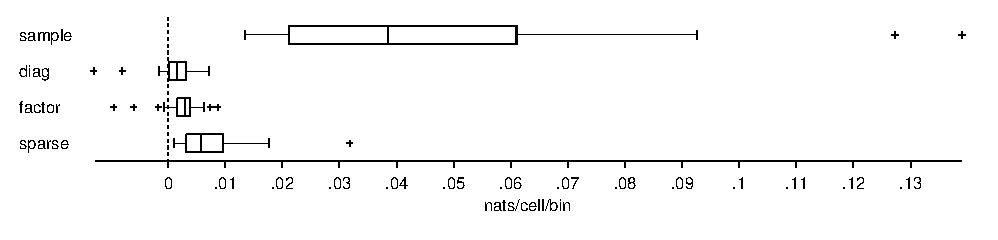
\includegraphics[width=\textwidth]{./figures/Figure3.eps}
        \end{center}
\begin{caption}[Evaluation of correlation estimators by cross-validation]
{\bf Performance of estimator $C_{\sf sparse+latent}$ with respect to the normal loss function (eq.~\ref{eq:loss}) relative to the other estimators: $C_{\sf sample}$, $C_{\sf diag}$, $C_{\sf factor}$, and $C_{\sf sparse}$.}
Covariance estimators $C_{\sf sample}$, $C_{\sf diag}$, $C_{\sf factor}$, and $C_{\sf sparse}$ produced consistently greater validation losses than $C_{\sf sparse+latent}$ ($p<0.01$ in each comparison, Wilcoxon signed rank test, $n=27$ sites in 14 mice). The box plots indicate the $25^{th}$, $50^{th}$, and $75^{th}$ percentiles with the whiskers extending to the minimum and maximum values after excluding the outliers marked with `+'.
\end{caption}\label{fig:3}
\end{fullpage}
\end{figure}
